\documentclass[12pt]{article}

\usepackage[utf8]{inputenc}
\usepackage{geometry}
\geometry{a4paper,scale=0.75}
\linespread{1.5}
\usepackage{graphicx} 
\usepackage{float} 
\usepackage{subfig} 
\usepackage{enumerate}
\usepackage{enumitem}
\usepackage{amsmath}
\usepackage{array}
\usepackage{booktabs}
\usepackage{multirow}
\usepackage{amsfonts}
\usepackage[english]{babel}
\usepackage{amsthm}
\usepackage{dcolumn}
\usepackage{multicol}
\usepackage{stfloats}
\usepackage{lscape}
\usepackage[figuresright]{rotating}
\RequirePackage{pdflscape}
\usepackage[toc,page]{appendix}
\usepackage{geometry}
\usepackage{longtable}
\usepackage{comment}
\usepackage{xcolor}

% -------- enumerated sub-labels (a), (b), … --
\usepackage{enumitem}
\setlist[enumerate,1]{label=(\alph*),ref=\alph*}
% ---------------------------------------------

\usepackage{hyperref}
\hypersetup{hidelinks,
	colorlinks=true,
	allcolors=black,
	pdfstartview=Fit,
	breaklinks=true}
\usepackage{csquotes}
\usepackage{natbib}
\bibliographystyle{apalike}
\newtheorem{definition}{Definition}
\newtheorem{theorem}{Theorem}
\newtheorem{proposition}[theorem]{Proposition}
\newtheorem{lemma}[theorem]{Lemma}
\newtheorem{corollary}[theorem]{Corollary}
\newtheorem*{remark}{Remark}
\newtheorem{example}{Example}
\newtheorem{exercise}{Exercise}
\newtheorem{assumption}{Assumption}[section] % number within sections


\begin{document}

\begin{center}
    ECON 3123: Macroeconomic Theory I\\
    {\large \textbf{Tutorial Note 4: Basic IS-LM Framework}}\\
    Teaching Assistant: Harlly Zhou
\end{center}

\subsection*{Derivation of IS-LM Model}
Recall that in the goods market, the deamnd for goods is
\[ Z = C + I + G. \]
Recall that consumption depends on disposable income $Y-T$. And in reality, investment depends on output and interest rate:
\[ I = I (Y,i),\]
where $I$ increases with $Y$ and decreases with $i$. (Think about the intuition.)

Then we rewrite the demand as
\[ Z = C(Y-T) + I(Y,i) + G.\]
At equilibrium, we have
\[ Y = Z.\]
This determines the equilibrium output $Y^*$. When the nominal interest rate increases, the investment will decrease, shifting the $ZZ$ curve downwards. We have the new equilibrium output $Y'$, shown as Figure \ref{fig:is_01}.

\begin{figure}[htp]
    \centering
    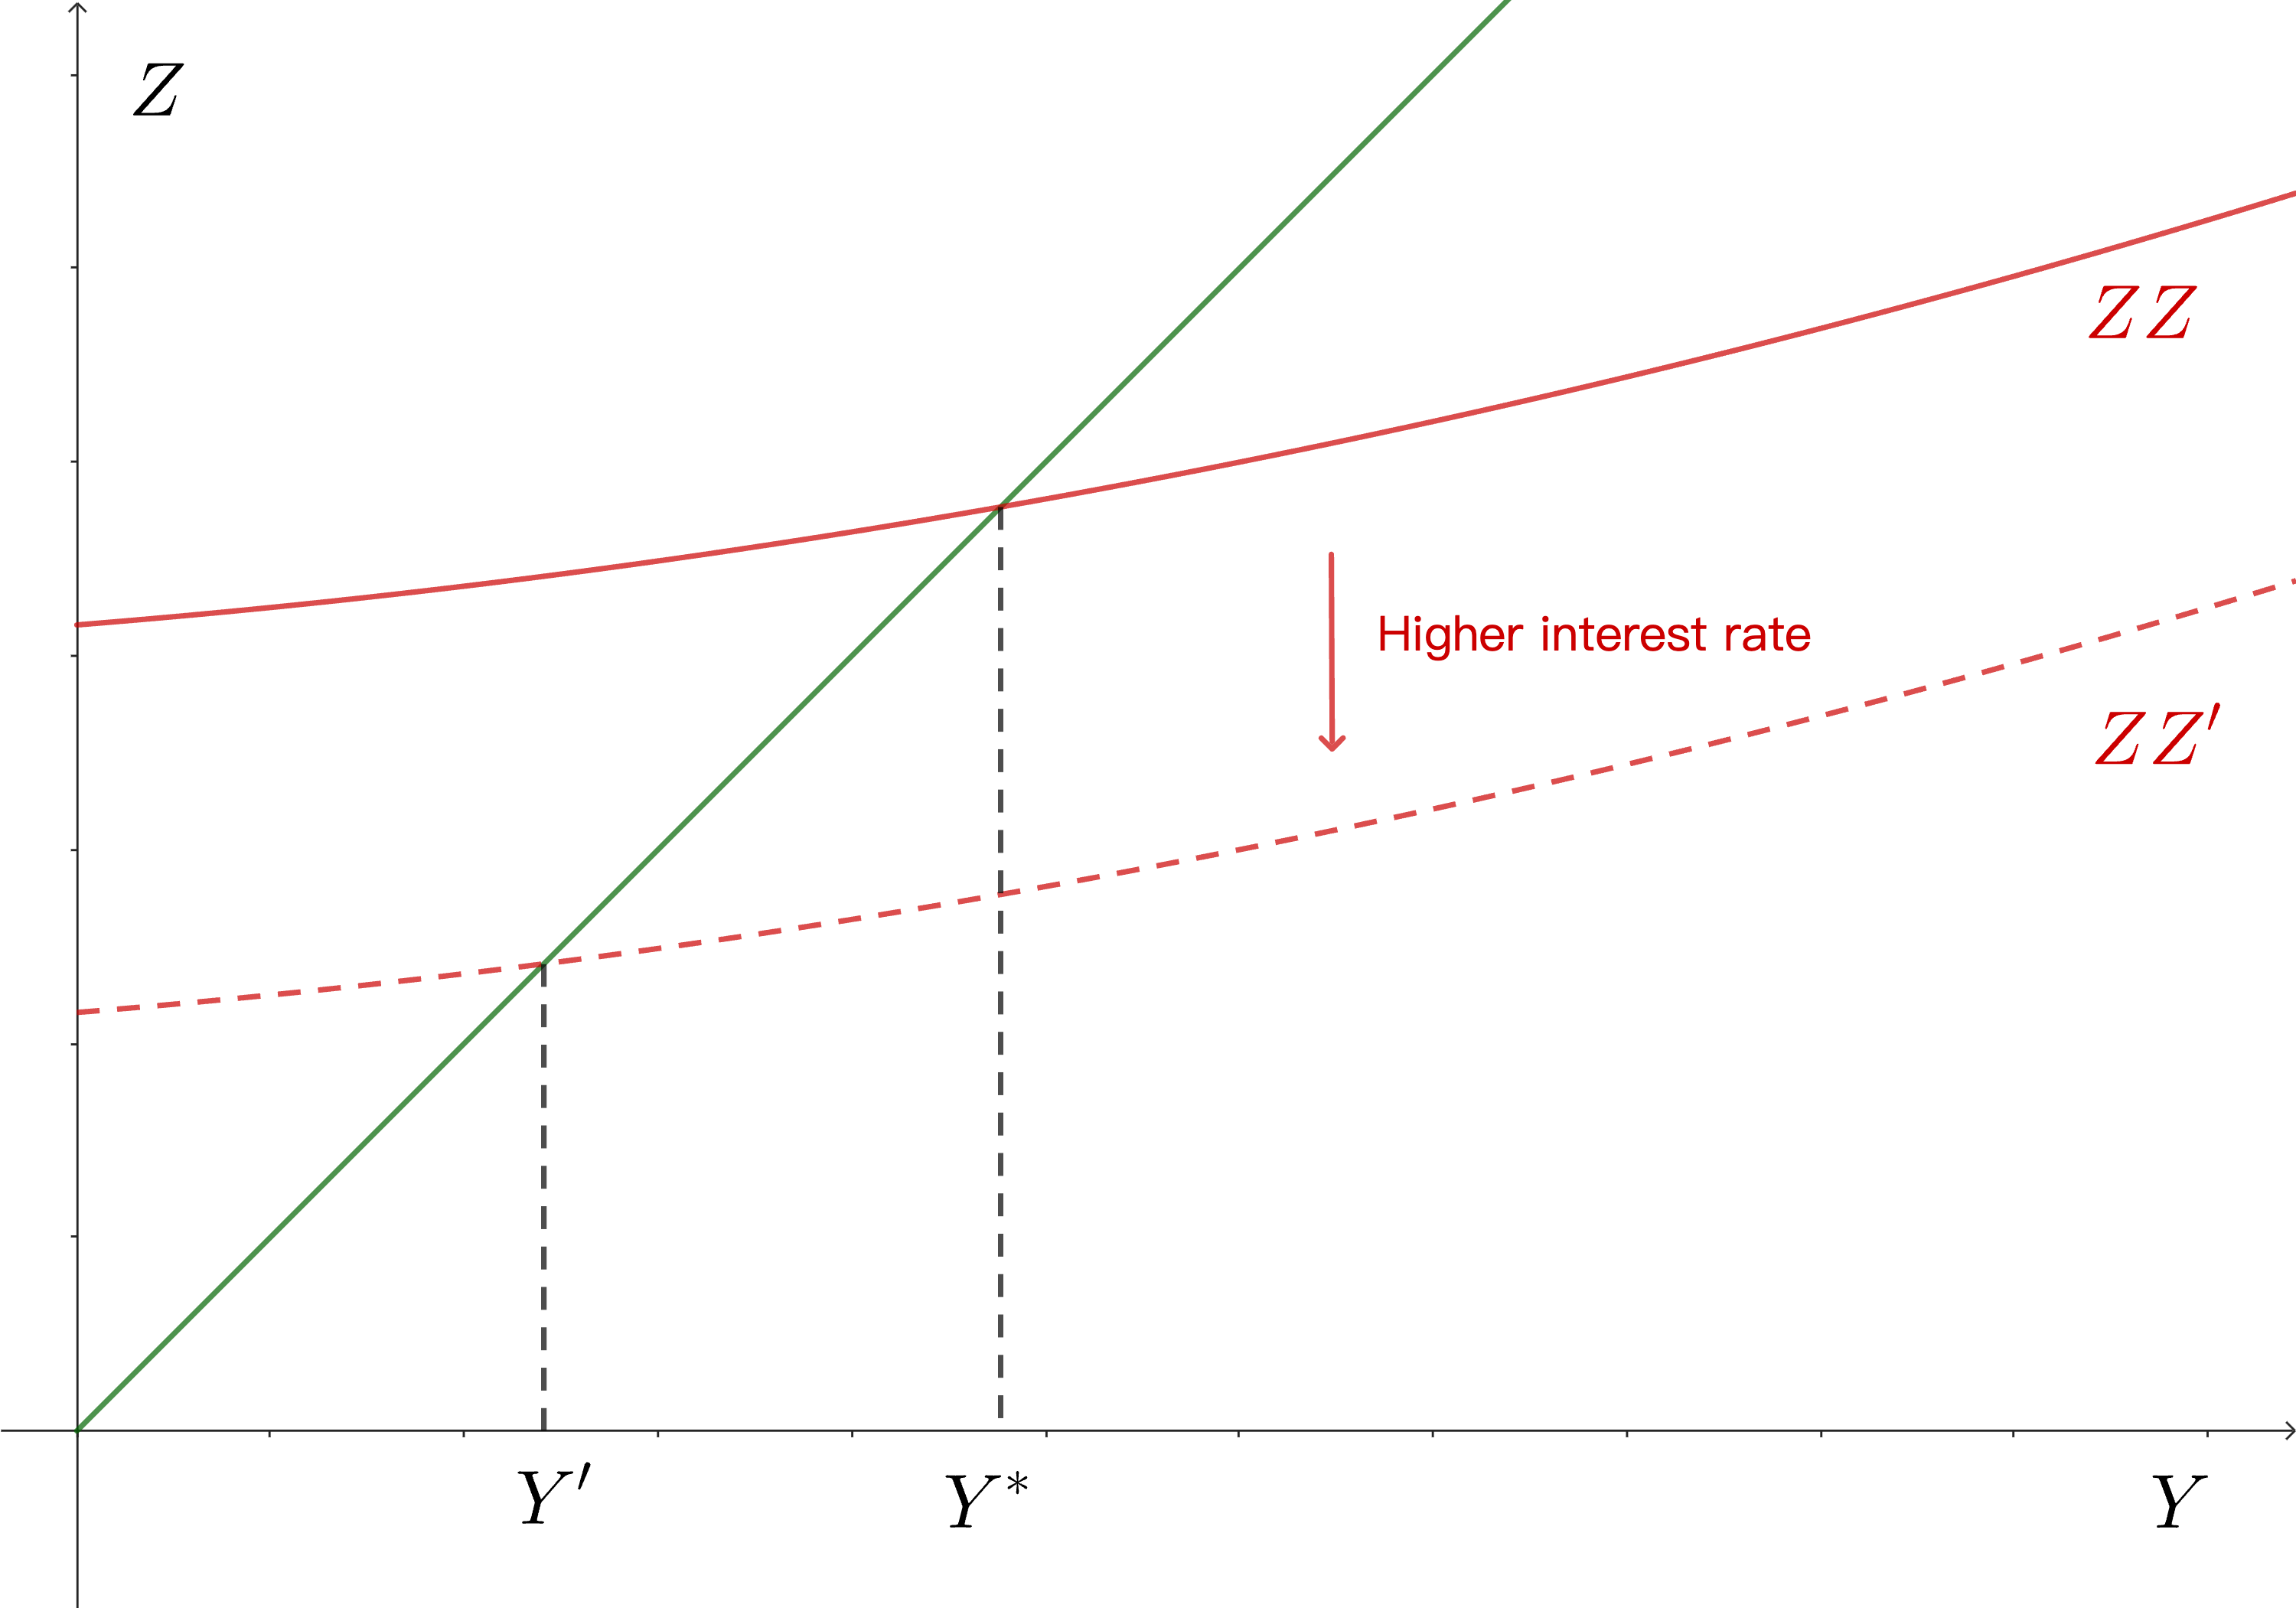
\includegraphics[width=0.6\textwidth]{is_01.png}
    \caption{Goods Market Equilibrium}
    \label{fig:is_01}
\end{figure}

If we put the interest rate and the output together, then we get the IS relation (Figrue \ref{fig:is_02}).\

\begin{figure}[htp]
    \centering
    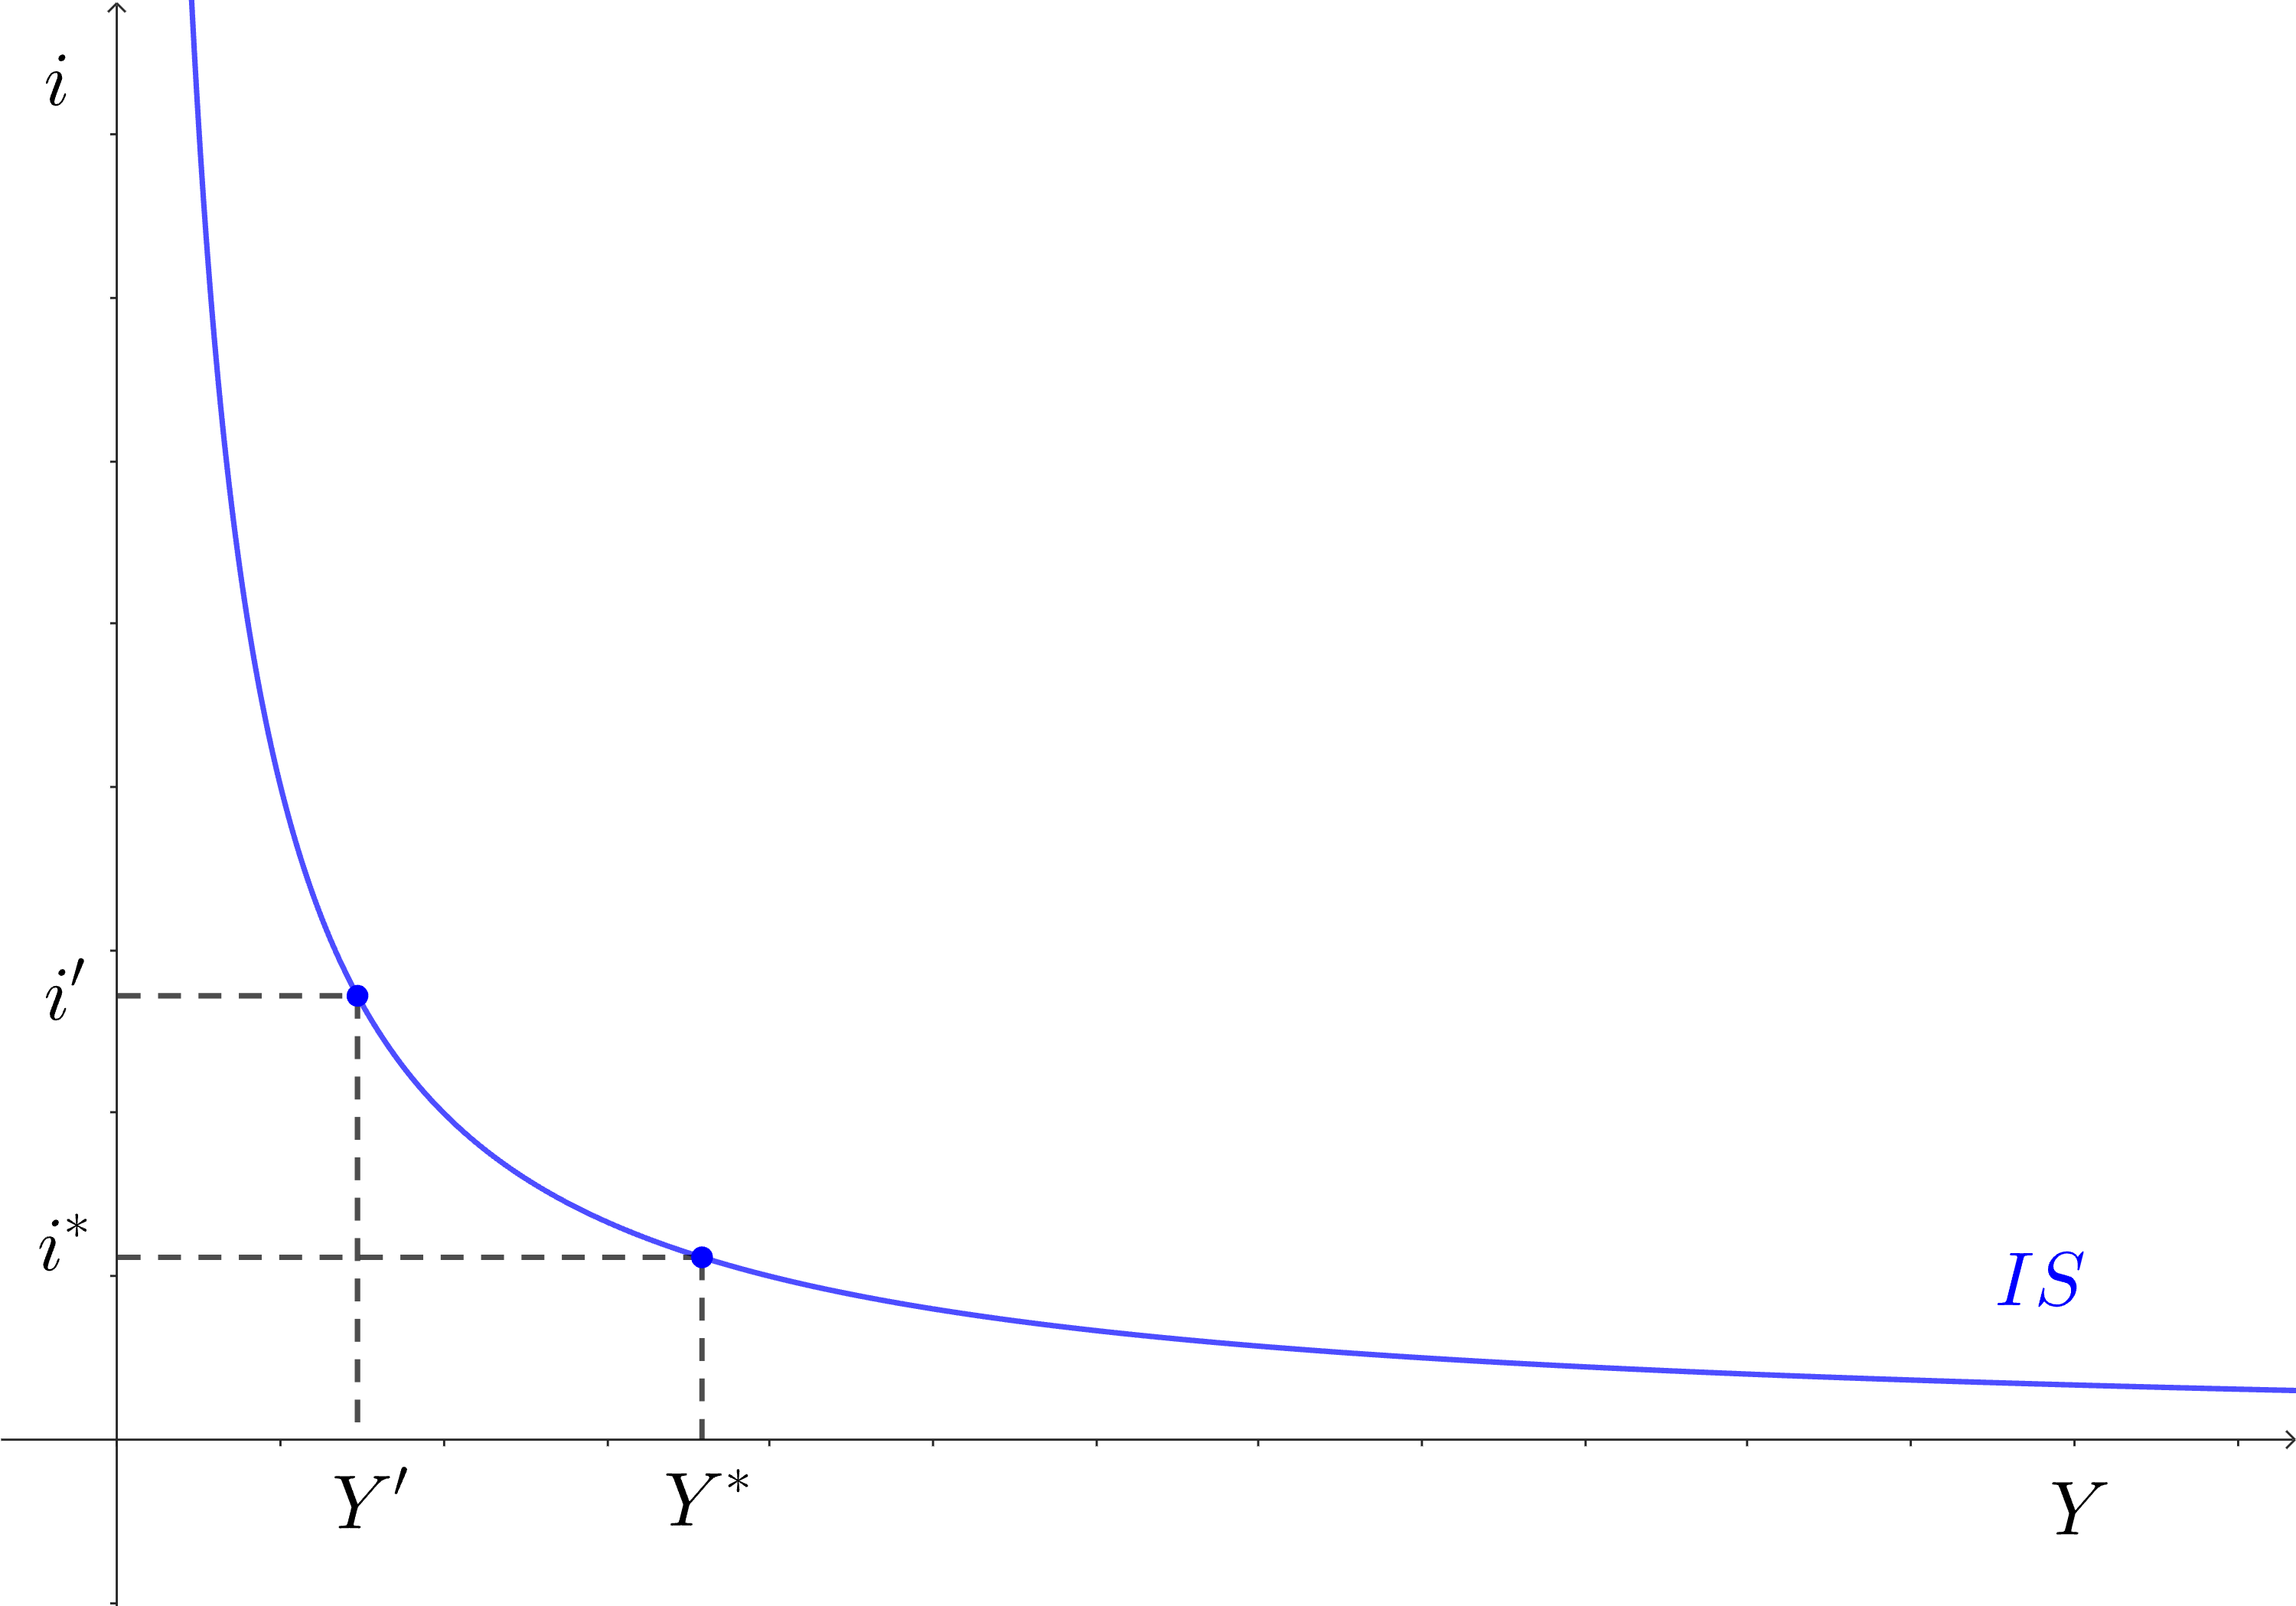
\includegraphics[width=0.6\textwidth]{is_02.png}
    \caption{Deriving IS curve from goods market equilibrium}
    \label{fig:is_02}
\end{figure}

Note that all the pairs $(i, Y)$ is a pair of \textbf{equilibrium} values of nominal interest and output.
\end{document}